% Options for packages loaded elsewhere
\PassOptionsToPackage{unicode}{hyperref}
\PassOptionsToPackage{hyphens}{url}
%
\documentclass[
]{article}
\usepackage{lmodern}
\usepackage{amssymb,amsmath}
\usepackage{ifxetex,ifluatex}
\ifnum 0\ifxetex 1\fi\ifluatex 1\fi=0 % if pdftex
  \usepackage[T1]{fontenc}
  \usepackage[utf8]{inputenc}
  \usepackage{textcomp} % provide euro and other symbols
\else % if luatex or xetex
  \usepackage{unicode-math}
  \defaultfontfeatures{Scale=MatchLowercase}
  \defaultfontfeatures[\rmfamily]{Ligatures=TeX,Scale=1}
\fi
% Use upquote if available, for straight quotes in verbatim environments
\IfFileExists{upquote.sty}{\usepackage{upquote}}{}
\IfFileExists{microtype.sty}{% use microtype if available
  \usepackage[]{microtype}
  \UseMicrotypeSet[protrusion]{basicmath} % disable protrusion for tt fonts
}{}
\makeatletter
\@ifundefined{KOMAClassName}{% if non-KOMA class
  \IfFileExists{parskip.sty}{%
    \usepackage{parskip}
  }{% else
    \setlength{\parindent}{0pt}
    \setlength{\parskip}{6pt plus 2pt minus 1pt}}
}{% if KOMA class
  \KOMAoptions{parskip=half}}
\makeatother
\usepackage{xcolor}
\IfFileExists{xurl.sty}{\usepackage{xurl}}{} % add URL line breaks if available
\IfFileExists{bookmark.sty}{\usepackage{bookmark}}{\usepackage{hyperref}}
\hypersetup{
  pdftitle={Calibrating a 3-state cancer model},
  pdfauthor={The DARTH workgroup},
  hidelinks,
  pdfcreator={LaTeX via pandoc}}
\urlstyle{same} % disable monospaced font for URLs
\usepackage[margin=1in]{geometry}
\usepackage{color}
\usepackage{fancyvrb}
\newcommand{\VerbBar}{|}
\newcommand{\VERB}{\Verb[commandchars=\\\{\}]}
\DefineVerbatimEnvironment{Highlighting}{Verbatim}{commandchars=\\\{\}}
% Add ',fontsize=\small' for more characters per line
\usepackage{framed}
\definecolor{shadecolor}{RGB}{248,248,248}
\newenvironment{Shaded}{\begin{snugshade}}{\end{snugshade}}
\newcommand{\AlertTok}[1]{\textcolor[rgb]{0.94,0.16,0.16}{#1}}
\newcommand{\AnnotationTok}[1]{\textcolor[rgb]{0.56,0.35,0.01}{\textbf{\textit{#1}}}}
\newcommand{\AttributeTok}[1]{\textcolor[rgb]{0.77,0.63,0.00}{#1}}
\newcommand{\BaseNTok}[1]{\textcolor[rgb]{0.00,0.00,0.81}{#1}}
\newcommand{\BuiltInTok}[1]{#1}
\newcommand{\CharTok}[1]{\textcolor[rgb]{0.31,0.60,0.02}{#1}}
\newcommand{\CommentTok}[1]{\textcolor[rgb]{0.56,0.35,0.01}{\textit{#1}}}
\newcommand{\CommentVarTok}[1]{\textcolor[rgb]{0.56,0.35,0.01}{\textbf{\textit{#1}}}}
\newcommand{\ConstantTok}[1]{\textcolor[rgb]{0.00,0.00,0.00}{#1}}
\newcommand{\ControlFlowTok}[1]{\textcolor[rgb]{0.13,0.29,0.53}{\textbf{#1}}}
\newcommand{\DataTypeTok}[1]{\textcolor[rgb]{0.13,0.29,0.53}{#1}}
\newcommand{\DecValTok}[1]{\textcolor[rgb]{0.00,0.00,0.81}{#1}}
\newcommand{\DocumentationTok}[1]{\textcolor[rgb]{0.56,0.35,0.01}{\textbf{\textit{#1}}}}
\newcommand{\ErrorTok}[1]{\textcolor[rgb]{0.64,0.00,0.00}{\textbf{#1}}}
\newcommand{\ExtensionTok}[1]{#1}
\newcommand{\FloatTok}[1]{\textcolor[rgb]{0.00,0.00,0.81}{#1}}
\newcommand{\FunctionTok}[1]{\textcolor[rgb]{0.00,0.00,0.00}{#1}}
\newcommand{\ImportTok}[1]{#1}
\newcommand{\InformationTok}[1]{\textcolor[rgb]{0.56,0.35,0.01}{\textbf{\textit{#1}}}}
\newcommand{\KeywordTok}[1]{\textcolor[rgb]{0.13,0.29,0.53}{\textbf{#1}}}
\newcommand{\NormalTok}[1]{#1}
\newcommand{\OperatorTok}[1]{\textcolor[rgb]{0.81,0.36,0.00}{\textbf{#1}}}
\newcommand{\OtherTok}[1]{\textcolor[rgb]{0.56,0.35,0.01}{#1}}
\newcommand{\PreprocessorTok}[1]{\textcolor[rgb]{0.56,0.35,0.01}{\textit{#1}}}
\newcommand{\RegionMarkerTok}[1]{#1}
\newcommand{\SpecialCharTok}[1]{\textcolor[rgb]{0.00,0.00,0.00}{#1}}
\newcommand{\SpecialStringTok}[1]{\textcolor[rgb]{0.31,0.60,0.02}{#1}}
\newcommand{\StringTok}[1]{\textcolor[rgb]{0.31,0.60,0.02}{#1}}
\newcommand{\VariableTok}[1]{\textcolor[rgb]{0.00,0.00,0.00}{#1}}
\newcommand{\VerbatimStringTok}[1]{\textcolor[rgb]{0.31,0.60,0.02}{#1}}
\newcommand{\WarningTok}[1]{\textcolor[rgb]{0.56,0.35,0.01}{\textbf{\textit{#1}}}}
\usepackage{graphicx,grffile}
\makeatletter
\def\maxwidth{\ifdim\Gin@nat@width>\linewidth\linewidth\else\Gin@nat@width\fi}
\def\maxheight{\ifdim\Gin@nat@height>\textheight\textheight\else\Gin@nat@height\fi}
\makeatother
% Scale images if necessary, so that they will not overflow the page
% margins by default, and it is still possible to overwrite the defaults
% using explicit options in \includegraphics[width, height, ...]{}
\setkeys{Gin}{width=\maxwidth,height=\maxheight,keepaspectratio}
% Set default figure placement to htbp
\makeatletter
\def\fps@figure{htbp}
\makeatother
\setlength{\emergencystretch}{3em} % prevent overfull lines
\providecommand{\tightlist}{%
  \setlength{\itemsep}{0pt}\setlength{\parskip}{0pt}}
\setcounter{secnumdepth}{-\maxdimen} % remove section numbering

\title{Calibrating a 3-state cancer model}
\usepackage{etoolbox}
\makeatletter
\providecommand{\subtitle}[1]{% add subtitle to \maketitle
  \apptocmd{\@title}{\par {\large #1 \par}}{}{}
}
\makeatother
\subtitle{Incremental mixture importance sampling (IMIS)}
\author{The DARTH workgroup}
\date{}

\begin{document}
\maketitle

Developed by the Decision Analysis in R for Technologies in Health
(DARTH) workgroup:

Fernando Alarid-Escudero, PhD (1)

Eva A. Enns, MS, PhD (2)

M.G. Myriam Hunink, MD, PhD (3,4)

Hawre J. Jalal, MD, PhD (5)

Eline M. Krijkamp, MSc (3)

Petros Pechlivanoglou, PhD (6)

Alan Yang, MSc (7)

In collaboration of:

\begin{enumerate}
\def\labelenumi{\arabic{enumi}.}
\tightlist
\item
  Division of Public Administration, Center for Research and Teaching in
  Economics (CIDE), Aguascalientes, Mexico
\item
  University of Minnesota School of Public Health, Minneapolis, MN, USA
\item
  Erasmus MC, Rotterdam, The Netherlands
\item
  Harvard T.H. Chan School of Public Health, Boston, USA
\item
  University of Pittsburgh Graduate School of Public Health, Pittsburgh,
  PA, USA
\item
  The Hospital for Sick Children, Toronto and University of Toronto,
  Toronto ON, Canada
\item
  The Hospital for Sick Children, Toronto ON, Canada
\end{enumerate}

Please cite our publications when using this code:

\begin{itemize}
\item
  Alarid-Escudero F, Maclehose RF, Peralta Y, Kuntz KM, Enns EA.
  Non-identifiability in model calibration and implications for medical
  decision making. Med Decis Making. 2018; 38(7):810-821.
  \url{https://pubmed.ncbi.nlm.nih.gov/30248276/}
\item
  Jalal H, Pechlivanoglou P, Krijkamp E, Alarid-Escudero F, Enns E,
  Hunink MG. An Overview of R in Health Decision Sciences. Med Decis
  Making. 2017; 37(3): 735-746.
  \url{https://journals.sagepub.com/doi/abs/10.1177/0272989X16686559}
\end{itemize}

A walkthrough of the code could be found in the following link: -
\url{https://darth-git.github.io/calibSMDM2018-materials/}

Copyright 2017, THE HOSPITAL FOR SICK CHILDREN AND THE COLLABORATING
INSTITUTIONS. All rights reserved in Canada, the United States and
worldwide. Copyright, trademarks, trade names and any and all associated
intellectual property are exclusively owned by THE HOSPITAL FOR Sick
CHILDREN and the collaborating institutions. These materials may be
used, reproduced, modified, distributed and adapted with proper
attribution.

\newpage

\begin{Shaded}
\begin{Highlighting}[]
\KeywordTok{rm}\NormalTok{(}\DataTypeTok{list =} \KeywordTok{ls}\NormalTok{())      }\CommentTok{# clear memory (removes all the variables from the workspace)}
\end{Highlighting}
\end{Shaded}

\hypertarget{calibration-specifications}{%
\section{00 Calibration
Specifications}\label{calibration-specifications}}

Model: 3-State Cancer Relative Survival (CRS) Markov Model

Inputs to be calibrated: p\_Mets, p\_DieMets

Targets: Surv

Calibration method: Incremental mixture importance sampling (IMIS)

Goodness-of-fit measure: Sum of Log-Likelihood

\hypertarget{load-packages}{%
\section{01 Load packages}\label{load-packages}}

\begin{Shaded}
\begin{Highlighting}[]
\ControlFlowTok{if}\NormalTok{ (}\OperatorTok{!}\KeywordTok{require}\NormalTok{(}\StringTok{'pacman'}\NormalTok{)) \{}
  \KeywordTok{install.packages}\NormalTok{(}\StringTok{'pacman'}\NormalTok{)}
\NormalTok{\}}
\KeywordTok{library}\NormalTok{(pacman) }\CommentTok{# use this package to conveniently install other packages}
\CommentTok{# load (install if required) packages from CRAN}
\KeywordTok{p_load}\NormalTok{(}\StringTok{"lhs"}\NormalTok{, }\StringTok{"IMIS"}\NormalTok{, }\StringTok{"matrixStats"}\NormalTok{, }\StringTok{"plotrix"}\NormalTok{, }\StringTok{"psych"}\NormalTok{)  }
\end{Highlighting}
\end{Shaded}

\hypertarget{load-target-data}{%
\section{02 Load target data}\label{load-target-data}}

\begin{Shaded}
\begin{Highlighting}[]
\KeywordTok{load}\NormalTok{(}\StringTok{"CRS_CalibTargets.RData"}\NormalTok{)}
\NormalTok{lst_targets <-}\StringTok{ }\NormalTok{CRS_targets}

\CommentTok{# Plot the targets}

\CommentTok{# TARGET 1: Survival ("Surv")}
\NormalTok{plotrix}\OperatorTok{::}\KeywordTok{plotCI}\NormalTok{(}\DataTypeTok{x =}\NormalTok{ lst_targets}\OperatorTok{$}\NormalTok{Surv}\OperatorTok{$}\NormalTok{time, }\DataTypeTok{y =}\NormalTok{ lst_targets}\OperatorTok{$}\NormalTok{Surv}\OperatorTok{$}\NormalTok{value, }
                \DataTypeTok{ui =}\NormalTok{ lst_targets}\OperatorTok{$}\NormalTok{Surv}\OperatorTok{$}\NormalTok{ub,}
                \DataTypeTok{li =}\NormalTok{ lst_targets}\OperatorTok{$}\NormalTok{Surv}\OperatorTok{$}\NormalTok{lb,}
                \DataTypeTok{ylim =} \KeywordTok{c}\NormalTok{(}\DecValTok{0}\NormalTok{, }\DecValTok{1}\NormalTok{), }
                \DataTypeTok{xlab =} \StringTok{"Time"}\NormalTok{, }\DataTypeTok{ylab =} \StringTok{"Pr Survive"}\NormalTok{)}
\end{Highlighting}
\end{Shaded}

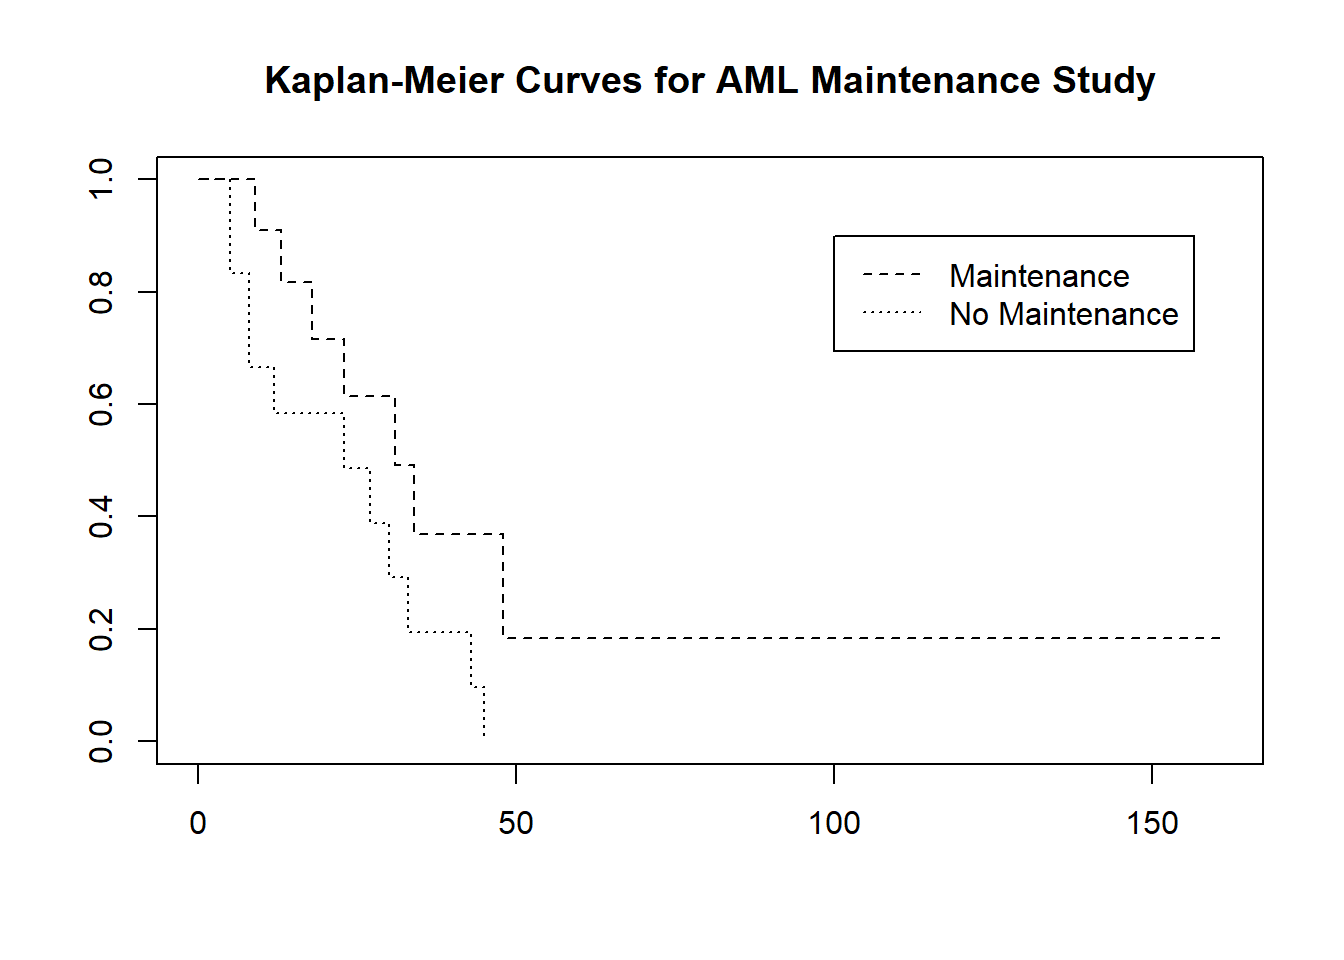
\includegraphics{CRS_Calib_IMIS_files/figure-latex/unnamed-chunk-3-1.pdf}

\begin{Shaded}
\begin{Highlighting}[]
\CommentTok{# TARGET 2: (if you had more...)}
\CommentTok{# plotrix::plotCI(x = lst_targets$Target2$time, y = lst_targets$Target2$value, }
\CommentTok{#                 ui = lst_targets$Target2$ub,}
\CommentTok{#                 li = lst_targets$Target2$lb,}
\CommentTok{#                 ylim = c(0, 1), }
\CommentTok{#                 xlab = "Time", ylab = "Target 2")}
\end{Highlighting}
\end{Shaded}

\hypertarget{load-model-as-a-function}{%
\section{03 Load model as a function}\label{load-model-as-a-function}}

\begin{Shaded}
\begin{Highlighting}[]
\CommentTok{# - inputs are parameters to be estimated through calibration}
\CommentTok{# - outputs correspond to the target data}

\KeywordTok{source}\NormalTok{(}\StringTok{"CRS_MarkovModel_Function.R"}\NormalTok{) }\CommentTok{# creates the function run_crs_markov()}

\CommentTok{# Check that it works}
\NormalTok{v_params_test <-}\StringTok{ }\KeywordTok{c}\NormalTok{(}\DataTypeTok{p_Mets =} \FloatTok{0.10}\NormalTok{, }\DataTypeTok{p_DieMets =} \FloatTok{0.05}\NormalTok{)}
\KeywordTok{run_crs_markov}\NormalTok{(v_params_test) }\CommentTok{# It works!}
\end{Highlighting}
\end{Shaded}

\begin{verbatim}
## $Surv
##          2          3          4          5          6          7          8 
## 0.99500000 0.98575000 0.97291250 0.95707188 0.93874278 0.91837769 0.89637365 
##          9         10         11         12         13         14         15 
## 0.87307833 0.84879544 0.82378959 0.79829064 0.77249758 0.74658203 0.72069133 
##         16         17         18         19         20         21         22 
## 0.69495132 0.66946885 0.64433400 0.61962203 0.59539519 0.57170426 0.54859000 
##         23         24         25         26         27         28         29 
## 0.52608435 0.50421161 0.48298935 0.46242937 0.44253844 0.42331901 0.40476980 
##         30         31         32         33         34         35         36 
## 0.38688637 0.36966161 0.35308613 0.33714867 0.32183639 0.30713521 0.29303003 
##         37         38         39         40         41         42         43 
## 0.27950495 0.26654348 0.25412871 0.24224343 0.23087030 0.21999193 0.20959096 
##         44         45         46         47         48         49         50 
## 0.19965017 0.19015255 0.18108132 0.17242001 0.16415250 0.15626300 0.14873618 
##         51         52         53         54         55         56         57 
## 0.14155706 0.13471112 0.12818429 0.12196293 0.11603386 0.11038433 0.10500206 
##         58         59         60 
## 0.09987521 0.09499237 0.09034259
\end{verbatim}

\hypertarget{specify-calibration-parameters}{%
\section{04 Specify calibration
parameters}\label{specify-calibration-parameters}}

\begin{Shaded}
\begin{Highlighting}[]
\CommentTok{# Specify seed (for reproducible sequence of random numbers)}
\KeywordTok{set.seed}\NormalTok{(}\DecValTok{072218}\NormalTok{)}

\CommentTok{# number of random samples}
\NormalTok{n_resamp <-}\StringTok{ }\DecValTok{1000}

\CommentTok{# names and number of input parameters to be calibrated}
\NormalTok{v_param_names <-}\StringTok{ }\KeywordTok{c}\NormalTok{(}\StringTok{"p_Mets"}\NormalTok{,}\StringTok{"p_DieMets"}\NormalTok{)}
\NormalTok{n_param <-}\StringTok{ }\KeywordTok{length}\NormalTok{(v_param_names)}

\CommentTok{# range on input search space}
\NormalTok{lb <-}\StringTok{ }\KeywordTok{c}\NormalTok{(}\DataTypeTok{p_Mets =} \FloatTok{0.04}\NormalTok{, }\DataTypeTok{p_DieMets =} \FloatTok{0.04}\NormalTok{) }\CommentTok{# lower bound}
\NormalTok{ub <-}\StringTok{ }\KeywordTok{c}\NormalTok{(}\DataTypeTok{p_Mets =} \FloatTok{0.16}\NormalTok{, }\DataTypeTok{p_DieMets =} \FloatTok{0.16}\NormalTok{) }\CommentTok{# upper bound}

\CommentTok{# number of calibration targets}
\NormalTok{v_target_names <-}\StringTok{ }\KeywordTok{c}\NormalTok{(}\StringTok{"Surv"}\NormalTok{)}
\NormalTok{n_target       <-}\StringTok{ }\KeywordTok{length}\NormalTok{(v_target_names)}
\end{Highlighting}
\end{Shaded}

\hypertarget{calibration-functions}{%
\section{05 Calibration functions}\label{calibration-functions}}

\begin{Shaded}
\begin{Highlighting}[]
\CommentTok{#  Write function to sample from prior}
\NormalTok{sample_prior <-}\StringTok{ }\ControlFlowTok{function}\NormalTok{(n_samp)\{}
\NormalTok{  m_lhs_unit   <-}\StringTok{ }\KeywordTok{randomLHS}\NormalTok{(}\DataTypeTok{n =}\NormalTok{ n_samp, }\DataTypeTok{k =}\NormalTok{ n_param)}
\NormalTok{  m_param_samp <-}\StringTok{ }\KeywordTok{matrix}\NormalTok{(}\DataTypeTok{nrow =}\NormalTok{ n_samp, }\DataTypeTok{ncol =}\NormalTok{ n_param)}
  \KeywordTok{colnames}\NormalTok{(m_param_samp) <-}\StringTok{ }\NormalTok{v_param_names}
  \ControlFlowTok{for}\NormalTok{ (i }\ControlFlowTok{in} \DecValTok{1}\OperatorTok{:}\NormalTok{n_param)\{}
\NormalTok{    m_param_samp[, i] <-}\StringTok{ }\KeywordTok{qunif}\NormalTok{(m_lhs_unit[,i],}
                               \DataTypeTok{min =}\NormalTok{ lb[i],}
                               \DataTypeTok{max =}\NormalTok{ ub[i])}
    \CommentTok{# ALTERNATIVE prior using beta (or other) distributions}
    \CommentTok{# m_param_samp[, i] <- qbeta(m_lhs_unit[,i],}
    \CommentTok{#                            shape1 = 1,}
    \CommentTok{#                            shape2 = 1)}
\NormalTok{  \}}
  \KeywordTok{return}\NormalTok{(m_param_samp)}
\NormalTok{\}}

\CommentTok{# view resulting parameter set samples}
\KeywordTok{pairs.panels}\NormalTok{(}\KeywordTok{sample_prior}\NormalTok{(}\DecValTok{1000}\NormalTok{))}
\end{Highlighting}
\end{Shaded}

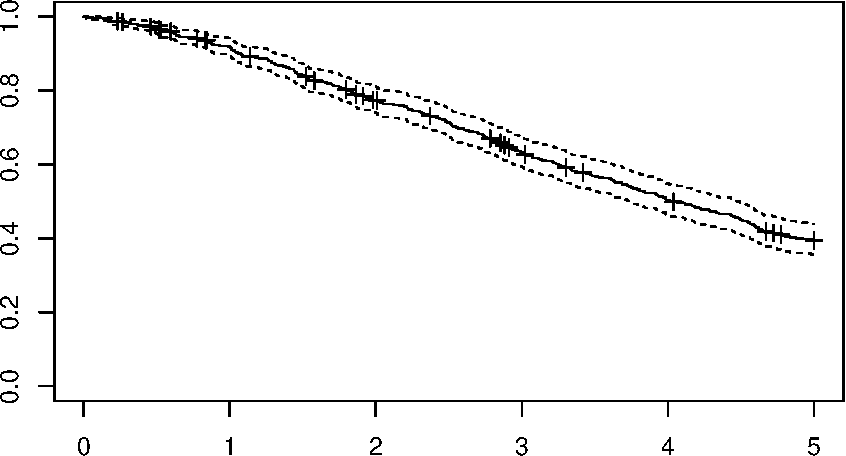
\includegraphics{CRS_Calib_IMIS_files/figure-latex/unnamed-chunk-6-1.pdf}

\begin{Shaded}
\begin{Highlighting}[]
\CommentTok{###  PRIOR  }\AlertTok{###}\CommentTok{ }
\CommentTok{# Write functions to evaluate log-prior and prior}

\CommentTok{# function that calculates the log-prior}
\NormalTok{calc_log_prior <-}\StringTok{ }\ControlFlowTok{function}\NormalTok{(v_params)\{}
  \ControlFlowTok{if}\NormalTok{(}\KeywordTok{is.null}\NormalTok{(}\KeywordTok{dim}\NormalTok{(v_params))) \{ }\CommentTok{# If vector, change to matrix}
\NormalTok{    v_params <-}\StringTok{ }\KeywordTok{t}\NormalTok{(v_params) }
\NormalTok{  \}}
\NormalTok{  n_samp <-}\StringTok{ }\KeywordTok{nrow}\NormalTok{(v_params)}
  \KeywordTok{colnames}\NormalTok{(v_params) <-}\StringTok{ }\NormalTok{v_param_names}
\NormalTok{  lprior <-}\StringTok{ }\KeywordTok{rep}\NormalTok{(}\DecValTok{0}\NormalTok{, n_samp)}
  \ControlFlowTok{for}\NormalTok{ (i }\ControlFlowTok{in} \DecValTok{1}\OperatorTok{:}\NormalTok{n_param)\{}
\NormalTok{    lprior <-}\StringTok{ }\NormalTok{lprior }\OperatorTok{+}\StringTok{ }\KeywordTok{dunif}\NormalTok{(v_params[, i],}
                             \DataTypeTok{min =}\NormalTok{ lb[i],}
                             \DataTypeTok{max =}\NormalTok{ ub[i], }
                             \DataTypeTok{log =}\NormalTok{ T)}
    \CommentTok{# ALTERNATIVE prior using beta distributions}
    \CommentTok{# lprior <- lprior + dbeta(v_params[, i],}
    \CommentTok{#                          shape1 = 1,}
    \CommentTok{#                          shape2 = 1, }
    \CommentTok{#                          log = T)}
\NormalTok{  \}}
  \KeywordTok{return}\NormalTok{(lprior)}
\NormalTok{\}}
\KeywordTok{calc_log_prior}\NormalTok{(}\DataTypeTok{v_params =}\NormalTok{ v_params_test)}
\end{Highlighting}
\end{Shaded}

\begin{verbatim}
##   p_Mets 
## 4.240527
\end{verbatim}

\begin{Shaded}
\begin{Highlighting}[]
\KeywordTok{calc_log_prior}\NormalTok{(}\DataTypeTok{v_params =} \KeywordTok{sample_prior}\NormalTok{(}\DecValTok{10}\NormalTok{))}
\end{Highlighting}
\end{Shaded}

\begin{verbatim}
##  [1] 4.240527 4.240527 4.240527 4.240527 4.240527 4.240527 4.240527 4.240527
##  [9] 4.240527 4.240527
\end{verbatim}

\begin{Shaded}
\begin{Highlighting}[]
\CommentTok{# function that calculates the (non-log) prior}
\NormalTok{calc_prior <-}\StringTok{ }\ControlFlowTok{function}\NormalTok{(v_params) \{ }
  \KeywordTok{exp}\NormalTok{(}\KeywordTok{calc_log_prior}\NormalTok{(v_params)) }
\NormalTok{\}}
\KeywordTok{calc_prior}\NormalTok{(}\DataTypeTok{v_params =}\NormalTok{ v_params_test)}
\end{Highlighting}
\end{Shaded}

\begin{verbatim}
##   p_Mets 
## 69.44444
\end{verbatim}

\begin{Shaded}
\begin{Highlighting}[]
\KeywordTok{calc_prior}\NormalTok{(}\DataTypeTok{v_params =} \KeywordTok{sample_prior}\NormalTok{(}\DecValTok{10}\NormalTok{))}
\end{Highlighting}
\end{Shaded}

\begin{verbatim}
##  [1] 69.44444 69.44444 69.44444 69.44444 69.44444 69.44444 69.44444 69.44444
##  [9] 69.44444 69.44444
\end{verbatim}

\begin{Shaded}
\begin{Highlighting}[]
\CommentTok{###  LIKELIHOOD  }\AlertTok{###}
\CommentTok{# Write functions to evaluate log-likelihood and likelihood}

\CommentTok{# function to calculate the log-likelihood}
\NormalTok{calc_log_lik <-}\StringTok{ }\ControlFlowTok{function}\NormalTok{(v_params)\{}
  \CommentTok{# par_vector: a vector (or matrix) of model parameters }
  \ControlFlowTok{if}\NormalTok{(}\KeywordTok{is.null}\NormalTok{(}\KeywordTok{dim}\NormalTok{(v_params))) \{ }\CommentTok{# If vector, change to matrix}
\NormalTok{    v_params <-}\StringTok{ }\KeywordTok{t}\NormalTok{(v_params) }
\NormalTok{  \}}
\NormalTok{  n_samp <-}\StringTok{ }\KeywordTok{nrow}\NormalTok{(v_params)}
\NormalTok{  v_llik <-}\StringTok{ }\KeywordTok{matrix}\NormalTok{(}\DecValTok{0}\NormalTok{, }\DataTypeTok{nrow =}\NormalTok{ n_samp, }\DataTypeTok{ncol =}\NormalTok{ n_target) }
\NormalTok{  llik_overall <-}\StringTok{ }\KeywordTok{numeric}\NormalTok{(n_samp)}
  \ControlFlowTok{for}\NormalTok{(j }\ControlFlowTok{in} \DecValTok{1}\OperatorTok{:}\NormalTok{n_samp) \{ }\CommentTok{# j=1}
\NormalTok{    jj <-}\StringTok{ }\KeywordTok{tryCatch}\NormalTok{( \{ }
      \CommentTok{###   Run model for parametr set "v_params" }\AlertTok{###}
\NormalTok{      model_res <-}\StringTok{ }\KeywordTok{run_crs_markov}\NormalTok{(v_params[j, ])}
      
      \CommentTok{###  Calculate log-likelihood of model outputs to targets  }\AlertTok{###}
      \CommentTok{# TARGET 1: Survival ("Surv")}
      \CommentTok{# log likelihood  }
\NormalTok{      v_llik[j, }\DecValTok{1}\NormalTok{] <-}\StringTok{ }\KeywordTok{sum}\NormalTok{(}\KeywordTok{dnorm}\NormalTok{(}\DataTypeTok{x =}\NormalTok{ lst_targets}\OperatorTok{$}\NormalTok{Surv}\OperatorTok{$}\NormalTok{value,}
                                \DataTypeTok{mean =}\NormalTok{ model_res}\OperatorTok{$}\NormalTok{Surv,}
                                \DataTypeTok{sd =}\NormalTok{ lst_targets}\OperatorTok{$}\NormalTok{Surv}\OperatorTok{$}\NormalTok{se,}
                                \DataTypeTok{log =}\NormalTok{ T))}
      
      \CommentTok{# TARGET 2: (if you had more...)}
      \CommentTok{# log likelihood}
      \CommentTok{# v_llik[j, 2] <- sum(dnorm(x = lst_targets$Target2$value,}
      \CommentTok{#                        mean = model_res$Target2,}
      \CommentTok{#                        sd = lst_targets$Target2$se,}
      \CommentTok{#                        log = T))}
      
      \CommentTok{# OVERALL }
\NormalTok{      llik_overall[j] <-}\StringTok{ }\KeywordTok{sum}\NormalTok{(v_llik[j, ])}
\NormalTok{    \}, }\DataTypeTok{error =} \ControlFlowTok{function}\NormalTok{(e) }\OtherTok{NA}\NormalTok{) }
    \ControlFlowTok{if}\NormalTok{(}\KeywordTok{is.na}\NormalTok{(jj)) \{ llik_overall <-}\StringTok{ }\OperatorTok{-}\OtherTok{Inf}\NormalTok{ \}}
\NormalTok{  \} }\CommentTok{# End loop over sampled parameter sets}
  \CommentTok{# return LLIK}
  \KeywordTok{return}\NormalTok{(llik_overall)}
\NormalTok{\}}
\KeywordTok{calc_log_lik}\NormalTok{(}\DataTypeTok{v_params =}\NormalTok{ v_params_test)}
\end{Highlighting}
\end{Shaded}

\begin{verbatim}
## [1] 142.7532
\end{verbatim}

\begin{Shaded}
\begin{Highlighting}[]
\KeywordTok{calc_log_lik}\NormalTok{(}\DataTypeTok{v_params =} \KeywordTok{sample_prior}\NormalTok{(}\DecValTok{10}\NormalTok{))}
\end{Highlighting}
\end{Shaded}

\begin{verbatim}
##  [1]  -745.91505   -22.67092 -1244.68778    88.75113  -323.23769   119.03787
##  [7] -1745.10789   106.42907  -115.02276  -290.51643
\end{verbatim}

\begin{Shaded}
\begin{Highlighting}[]
\CommentTok{# function to calculate the (non-log) likelihood}
\NormalTok{calc_likelihood <-}\StringTok{ }\ControlFlowTok{function}\NormalTok{(v_params)\{ }
  \KeywordTok{exp}\NormalTok{(}\KeywordTok{calc_log_lik}\NormalTok{(v_params)) }
\NormalTok{\}}
\KeywordTok{calc_likelihood}\NormalTok{(}\DataTypeTok{v_params =}\NormalTok{ v_params_test)}
\end{Highlighting}
\end{Shaded}

\begin{verbatim}
## [1] 9.929821e+61
\end{verbatim}

\begin{Shaded}
\begin{Highlighting}[]
\KeywordTok{calc_likelihood}\NormalTok{(}\DataTypeTok{v_params =} \KeywordTok{sample_prior}\NormalTok{(}\DecValTok{10}\NormalTok{))}
\end{Highlighting}
\end{Shaded}

\begin{verbatim}
##  [1]  0.000000e+00  0.000000e+00  3.713648e-79 6.819515e-195  1.245525e+61
##  [6]  4.361002e-64  1.332579e-99 5.048240e-115 2.040287e-108  0.000000e+00
\end{verbatim}

\begin{Shaded}
\begin{Highlighting}[]
\CommentTok{###  POSTERIOR  }\AlertTok{###}
\CommentTok{# Write functions to evaluate log-posterior and posterior}

\CommentTok{# function that calculates the log-posterior}
\NormalTok{calc_log_post <-}\StringTok{ }\ControlFlowTok{function}\NormalTok{(v_params) \{ }
\NormalTok{  lpost <-}\StringTok{ }\KeywordTok{calc_log_prior}\NormalTok{(v_params) }\OperatorTok{+}\StringTok{ }\KeywordTok{calc_log_lik}\NormalTok{(v_params)}
  \KeywordTok{return}\NormalTok{(lpost) }
\NormalTok{\}}
\KeywordTok{calc_log_post}\NormalTok{(}\DataTypeTok{v_params =}\NormalTok{ v_params_test)}
\end{Highlighting}
\end{Shaded}

\begin{verbatim}
##   p_Mets 
## 146.9938
\end{verbatim}

\begin{Shaded}
\begin{Highlighting}[]
\KeywordTok{calc_log_post}\NormalTok{(}\DataTypeTok{v_params =} \KeywordTok{sample_prior}\NormalTok{(}\DecValTok{10}\NormalTok{))}
\end{Highlighting}
\end{Shaded}

\begin{verbatim}
##  [1]  -103.90451  -689.80111   147.69552   101.63156  -629.16930 -1079.47013
##  [7] -1560.30601   127.95078  -693.87520    73.12498
\end{verbatim}

\begin{Shaded}
\begin{Highlighting}[]
\CommentTok{# function that calculates the (non-log) posterior}
\NormalTok{calc_post <-}\StringTok{ }\ControlFlowTok{function}\NormalTok{(v_params) \{ }
  \KeywordTok{exp}\NormalTok{(}\KeywordTok{calc_log_post}\NormalTok{(v_params)) }
\NormalTok{\}}
\KeywordTok{calc_post}\NormalTok{(}\DataTypeTok{v_params =}\NormalTok{ v_params_test)}
\end{Highlighting}
\end{Shaded}

\begin{verbatim}
##       p_Mets 
## 6.895709e+63
\end{verbatim}

\begin{Shaded}
\begin{Highlighting}[]
\KeywordTok{calc_post}\NormalTok{(}\DataTypeTok{v_params =} \KeywordTok{sample_prior}\NormalTok{(}\DecValTok{10}\NormalTok{))}
\end{Highlighting}
\end{Shaded}

\begin{verbatim}
##  [1] 9.617949e+56 0.000000e+00 5.127496e+53 3.865963e+52 1.881158e+65
##  [6] 2.355290e+64 0.000000e+00 2.117543e-95 0.000000e+00 0.000000e+00
\end{verbatim}

\hypertarget{calibrate}{%
\section{06 Calibrate!}\label{calibrate}}

\begin{Shaded}
\begin{Highlighting}[]
\CommentTok{# record start time of calibration}
\NormalTok{t_init <-}\StringTok{ }\KeywordTok{Sys.time}\NormalTok{()}

\CommentTok{###  Bayesian calibration using IMIS  }\AlertTok{###}
\CommentTok{# define three functions needed by IMIS: prior(x), likelihood(x), sample.prior(n)}
\NormalTok{prior <-}\StringTok{ }\NormalTok{calc_prior}
\NormalTok{likelihood <-}\StringTok{ }\NormalTok{calc_likelihood}
\NormalTok{sample.prior <-}\StringTok{ }\NormalTok{sample_prior}

\CommentTok{# run IMIS}
\NormalTok{fit_imis <-}\StringTok{ }\KeywordTok{IMIS}\NormalTok{(}\DataTypeTok{B =} \DecValTok{1000}\NormalTok{, }\CommentTok{# the incremental sample size at each iteration of IMIS}
                 \DataTypeTok{B.re =}\NormalTok{ n_resamp, }\CommentTok{# the desired posterior sample size}
                 \DataTypeTok{number_k =} \DecValTok{10}\NormalTok{, }\CommentTok{# the maximum number of iterations in IMIS}
                 \DataTypeTok{D =} \DecValTok{0}\NormalTok{) }
\end{Highlighting}
\end{Shaded}

\begin{verbatim}
## [1] "10000 likelihoods are evaluated in 0.05 minutes"
## [1] "Stage   MargLike   UniquePoint   MaxWeight   ESS"
## [1]   1.000 151.123 225.283   0.013 143.111
## [1]   2.000 151.005 358.059   0.015 216.393
## [1]   3.000 151.021 506.061   0.003 566.544
## [1]   4.000 151.055 603.928   0.003 780.559
## [1]    5.000  151.061  712.465    0.002 1281.614
\end{verbatim}

\begin{Shaded}
\begin{Highlighting}[]
\CommentTok{# obtain draws from posterior}
\NormalTok{m_calib_res <-}\StringTok{ }\NormalTok{fit_imis}\OperatorTok{$}\NormalTok{resample}

\CommentTok{# Calculate log-likelihood (overall fit) and posterior probability of each sample}
\NormalTok{m_calib_res <-}\StringTok{ }\KeywordTok{cbind}\NormalTok{(m_calib_res, }
                      \StringTok{"Overall_fit"}\NormalTok{ =}\StringTok{ }\KeywordTok{calc_log_lik}\NormalTok{(m_calib_res[,v_param_names]),}
                      \StringTok{"Posterior_prob"}\NormalTok{ =}\StringTok{ }\KeywordTok{calc_post}\NormalTok{(m_calib_res[,v_param_names]))}

\CommentTok{# normalize posterior probability}
\NormalTok{m_calib_res[,}\StringTok{"Posterior_prob"}\NormalTok{] <-}\StringTok{ }\NormalTok{m_calib_res[,}\StringTok{"Posterior_prob"}\NormalTok{]}\OperatorTok{/}\KeywordTok{sum}\NormalTok{(m_calib_res[,}\StringTok{"Posterior_prob"}\NormalTok{])}

\CommentTok{# Calculate computation time}
\NormalTok{comp_time <-}\StringTok{ }\KeywordTok{Sys.time}\NormalTok{() }\OperatorTok{-}\StringTok{ }\NormalTok{t_init}
\end{Highlighting}
\end{Shaded}

\hypertarget{exploring-posterior-distribution}{%
\section{07 Exploring posterior
distribution}\label{exploring-posterior-distribution}}

\begin{Shaded}
\begin{Highlighting}[]
\CommentTok{# Plot the 1000 draws from the posterior}
\NormalTok{v_post_color <-}\StringTok{ }\NormalTok{scales}\OperatorTok{::}\KeywordTok{rescale}\NormalTok{(m_calib_res[, }\StringTok{"Posterior_prob"}\NormalTok{])}
\KeywordTok{plot}\NormalTok{(m_calib_res,}
     \DataTypeTok{xlim =} \KeywordTok{c}\NormalTok{(lb[}\DecValTok{1}\NormalTok{], ub[}\DecValTok{1}\NormalTok{]), }\DataTypeTok{ylim =} \KeywordTok{c}\NormalTok{(lb[}\DecValTok{2}\NormalTok{], ub[}\DecValTok{2}\NormalTok{]),}
     \DataTypeTok{xlab =}\NormalTok{ v_param_names[}\DecValTok{1}\NormalTok{], }\DataTypeTok{ylab =}\NormalTok{ v_param_names[}\DecValTok{2}\NormalTok{],}
     \DataTypeTok{col =}\NormalTok{ scales}\OperatorTok{::}\KeywordTok{alpha}\NormalTok{(}\StringTok{"black"}\NormalTok{, v_post_color))}
\CommentTok{# add center of Gaussian components}
\KeywordTok{points}\NormalTok{(fit_imis}\OperatorTok{$}\NormalTok{center, }\DataTypeTok{col =} \StringTok{"red"}\NormalTok{, }\DataTypeTok{pch =} \DecValTok{8}\NormalTok{)}
\KeywordTok{legend}\NormalTok{(}\StringTok{"topright"}\NormalTok{, }\KeywordTok{c}\NormalTok{(}\StringTok{"Draws from posterior"}\NormalTok{, }\StringTok{"Center of Gaussian components"}\NormalTok{),}
       \DataTypeTok{col =} \KeywordTok{c}\NormalTok{(}\StringTok{"black"}\NormalTok{, }\StringTok{"red"}\NormalTok{), }\DataTypeTok{pch =} \KeywordTok{c}\NormalTok{(}\DecValTok{1}\NormalTok{, }\DecValTok{8}\NormalTok{))}
\end{Highlighting}
\end{Shaded}

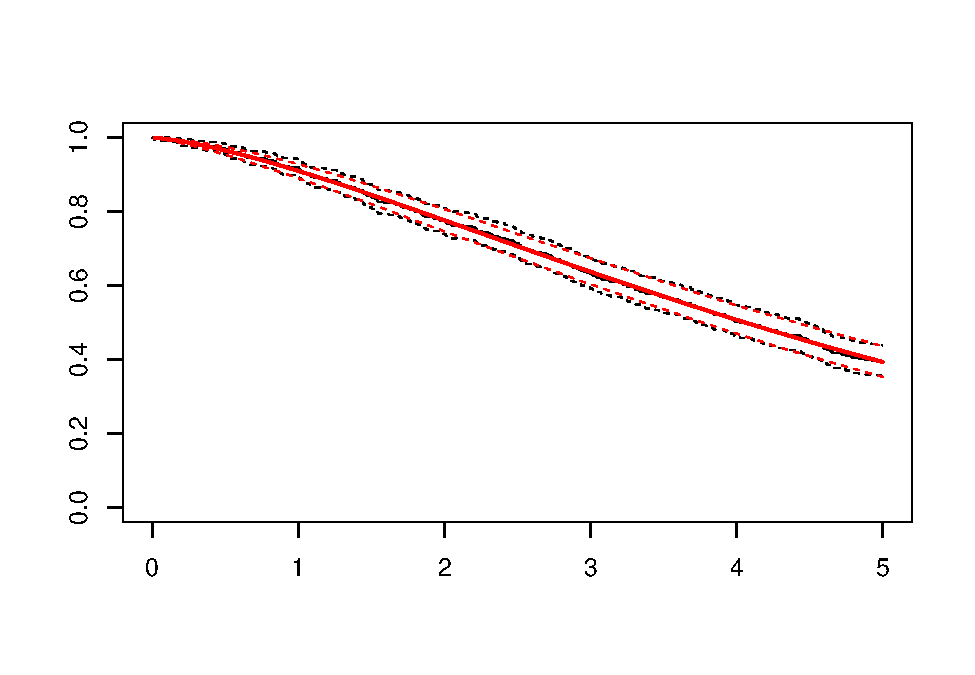
\includegraphics{CRS_Calib_IMIS_files/figure-latex/unnamed-chunk-8-1.pdf}

\begin{Shaded}
\begin{Highlighting}[]
\CommentTok{# Plot the 1000 draws from the posterior with marginal histograms}
\KeywordTok{pairs.panels}\NormalTok{(m_calib_res[,v_param_names])}
\end{Highlighting}
\end{Shaded}

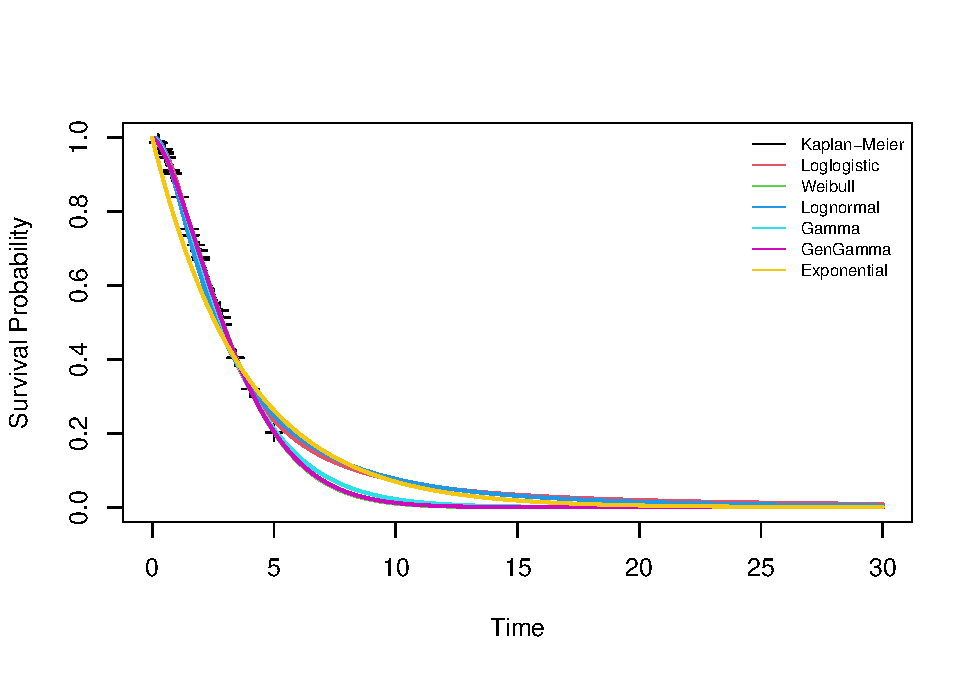
\includegraphics{CRS_Calib_IMIS_files/figure-latex/unnamed-chunk-8-2.pdf}

\begin{Shaded}
\begin{Highlighting}[]
\CommentTok{# Compute posterior mean}
\NormalTok{v_calib_post_mean <-}\StringTok{ }\KeywordTok{colMeans}\NormalTok{(m_calib_res[,v_param_names])}
\NormalTok{v_calib_post_mean}
\end{Highlighting}
\end{Shaded}

\begin{verbatim}
##     p_Mets  p_DieMets 
## 0.08611481 0.08582679
\end{verbatim}

\begin{Shaded}
\begin{Highlighting}[]
\CommentTok{# Compute posterior median and 95% credible interval}
\NormalTok{m_calib_res_95cr <-}\StringTok{ }\KeywordTok{colQuantiles}\NormalTok{(m_calib_res[,v_param_names], }\DataTypeTok{probs =} \KeywordTok{c}\NormalTok{(}\FloatTok{0.025}\NormalTok{, }\FloatTok{0.5}\NormalTok{, }\FloatTok{0.975}\NormalTok{))}
\NormalTok{m_calib_res_95cr}
\end{Highlighting}
\end{Shaded}

\begin{verbatim}
##                 2.5%        50%     97.5%
## p_Mets    0.04540699 0.09130227 0.1457041
## p_DieMets 0.04543305 0.05648003 0.1415877
\end{verbatim}

\begin{Shaded}
\begin{Highlighting}[]
\CommentTok{# Compute maximum-a-posteriori (MAP) parameter set}
\NormalTok{v_calib_map <-}\StringTok{ }\NormalTok{m_calib_res[}\KeywordTok{which.max}\NormalTok{(m_calib_res[,}\StringTok{"Posterior_prob"}\NormalTok{]),]}

\CommentTok{### Model-predicted output at mode/MAP }\AlertTok{###}
\NormalTok{v_out_best <-}\StringTok{ }\KeywordTok{run_crs_markov}\NormalTok{(v_calib_map[v_param_names])}
\end{Highlighting}
\end{Shaded}

\hypertarget{model-predicted-outputs-at-maximum-a-posteriori-map}{%
\subsection{07.1 Model predicted outputs at maximum-a-posteriori
(MAP)}\label{model-predicted-outputs-at-maximum-a-posteriori-map}}

\begin{Shaded}
\begin{Highlighting}[]
\CommentTok{### Plot model-predicted output at mode vs targets }\AlertTok{###}
\CommentTok{# set plot margins (helps plotting)}
\KeywordTok{par}\NormalTok{(}\DataTypeTok{mar=}\KeywordTok{c}\NormalTok{(}\DecValTok{5}\NormalTok{,}\DecValTok{4}\NormalTok{,}\DecValTok{4}\NormalTok{,}\DecValTok{4}\NormalTok{)) }
\CommentTok{# TARGET 1: Survival ("Surv")}
\NormalTok{plotrix}\OperatorTok{::}\KeywordTok{plotCI}\NormalTok{(}\DataTypeTok{x =}\NormalTok{ lst_targets}\OperatorTok{$}\NormalTok{Surv}\OperatorTok{$}\NormalTok{time, }\DataTypeTok{y =}\NormalTok{ lst_targets}\OperatorTok{$}\NormalTok{Surv}\OperatorTok{$}\NormalTok{value, }
                \DataTypeTok{ui =}\NormalTok{ lst_targets}\OperatorTok{$}\NormalTok{Surv}\OperatorTok{$}\NormalTok{ub,}
                \DataTypeTok{li =}\NormalTok{ lst_targets}\OperatorTok{$}\NormalTok{Surv}\OperatorTok{$}\NormalTok{lb,}
                \DataTypeTok{ylim =} \KeywordTok{c}\NormalTok{(}\DecValTok{0}\NormalTok{, }\DecValTok{1}\NormalTok{), }
                \DataTypeTok{xlab =} \StringTok{"Time"}\NormalTok{, }\DataTypeTok{ylab =} \StringTok{"Pr Survive"}\NormalTok{)}
\KeywordTok{points}\NormalTok{(}\DataTypeTok{x =}\NormalTok{ lst_targets}\OperatorTok{$}\NormalTok{Surv}\OperatorTok{$}\NormalTok{time, }
       \DataTypeTok{y =}\NormalTok{ v_out_best}\OperatorTok{$}\NormalTok{Surv, }
       \DataTypeTok{pch =} \DecValTok{8}\NormalTok{, }\DataTypeTok{col =} \StringTok{"red"}\NormalTok{)}
\KeywordTok{legend}\NormalTok{(}\StringTok{"topright"}\NormalTok{, }
       \DataTypeTok{legend =} \KeywordTok{c}\NormalTok{(}\StringTok{"Target"}\NormalTok{, }\StringTok{"Model-predicted output"}\NormalTok{),}
       \DataTypeTok{col =} \KeywordTok{c}\NormalTok{(}\StringTok{"black"}\NormalTok{, }\StringTok{"red"}\NormalTok{), }\DataTypeTok{pch =} \KeywordTok{c}\NormalTok{(}\DecValTok{1}\NormalTok{, }\DecValTok{8}\NormalTok{))}
\end{Highlighting}
\end{Shaded}

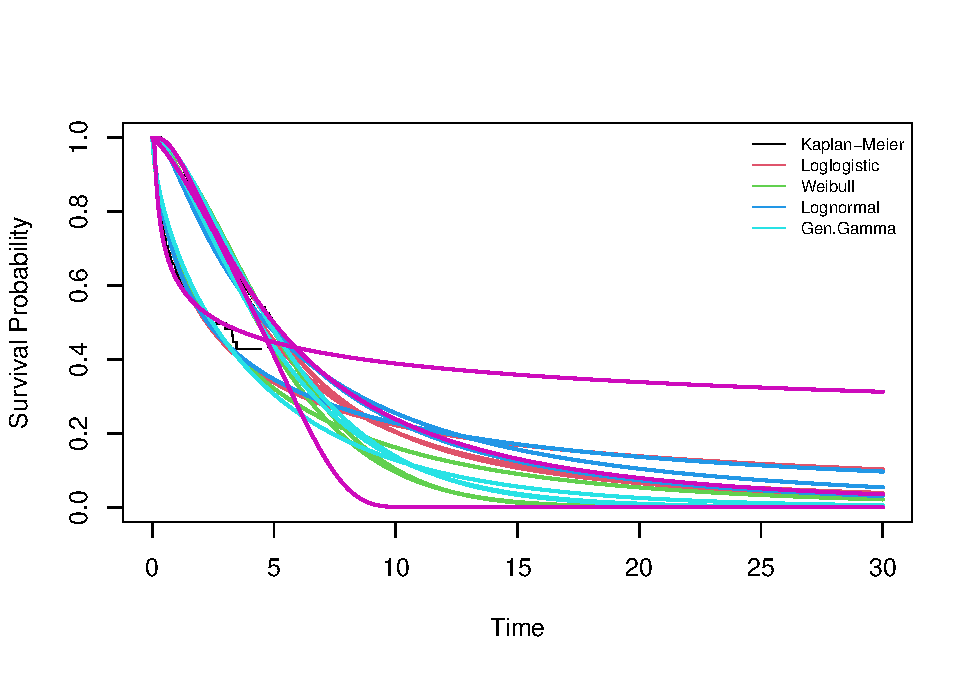
\includegraphics{CRS_Calib_IMIS_files/figure-latex/unnamed-chunk-9-1.pdf}

\begin{Shaded}
\begin{Highlighting}[]
\CommentTok{# TARGET 2: (if you had more...)}
\CommentTok{# plotrix::plotCI(x = lst_targets$Target2$time, y = lst_targets$Target2$value, }
\CommentTok{#                 ui = lst_targets$Target2$ub,}
\CommentTok{#                 li = lst_targets$Target2$lb,}
\CommentTok{#                 ylim = c(0, 1), }
\CommentTok{#                 xlab = "Time", ylab = "Target 2")}
\CommentTok{# points(x = lst_targets$Target2$time, }
\CommentTok{#        y = v_out_best$Target2, }
\CommentTok{#        pch = 8, col = "red")}
\CommentTok{# legend("topright", }
\CommentTok{#        legend = c("Target", "Model-predicted output"),}
\CommentTok{#        col = c("black", "red"), pch = c(1, 8))}
\end{Highlighting}
\end{Shaded}

\hypertarget{distribution-of-model-predicted-outputs}{%
\subsection{07.2 Distribution of model-predicted
outputs}\label{distribution-of-model-predicted-outputs}}

\begin{Shaded}
\begin{Highlighting}[]
\CommentTok{### Distribution of model-predicted output at mode vs targets }\AlertTok{###}
\CommentTok{## Initialize matrix to store outputs}
\NormalTok{m_out_post <-}\StringTok{ }\KeywordTok{matrix}\NormalTok{(}\OtherTok{NA}\NormalTok{, }
                     \DataTypeTok{nrow =}\NormalTok{ n_resamp, }
                     \DataTypeTok{ncol =} \KeywordTok{length}\NormalTok{(v_out_best}\OperatorTok{$}\NormalTok{Surv))}
\CommentTok{## Iterate model over all parameter sets from posterior distribution}
\ControlFlowTok{for}\NormalTok{(i }\ControlFlowTok{in} \DecValTok{1}\OperatorTok{:}\NormalTok{n_resamp)\{}
\NormalTok{  l_out <-}\StringTok{ }\KeywordTok{run_crs_markov}\NormalTok{(m_calib_res[i, ])}
\NormalTok{  m_out_post[i, ] <-}\StringTok{ }\NormalTok{l_out}\OperatorTok{$}\NormalTok{Surv}
  
  \ControlFlowTok{if}\NormalTok{(i}\OperatorTok{/}\NormalTok{(n_resamp}\OperatorTok{/}\DecValTok{10}\NormalTok{) }\OperatorTok{==}\StringTok{ }\KeywordTok{round}\NormalTok{(i}\OperatorTok{/}\NormalTok{(n_resamp}\OperatorTok{/}\DecValTok{10}\NormalTok{),}\DecValTok{0}\NormalTok{)) \{ }\CommentTok{# display progress every 10%}
    \KeywordTok{cat}\NormalTok{(}\StringTok{'}\CharTok{\textbackslash{}r}\StringTok{'}\NormalTok{, }\KeywordTok{paste}\NormalTok{(i}\OperatorTok{/}\NormalTok{n_resamp }\OperatorTok{*}\StringTok{ }\DecValTok{100}\NormalTok{, }\StringTok{"% done"}\NormalTok{, }\DataTypeTok{sep =} \StringTok{" "}\NormalTok{))}
\NormalTok{  \}}
\NormalTok{\}}
\end{Highlighting}
\end{Shaded}

\begin{verbatim}
##  10 % done 20 % done 30 % done 40 % done 50 % done 60 % done 70 % done 80 % done 90 % done 100 % done
\end{verbatim}

\begin{Shaded}
\begin{Highlighting}[]
\CommentTok{## Compute model-predicted posterior summary statistics}
\CommentTok{# Model-predicted posterior mean}
\NormalTok{v_out_post_mean      <-}\StringTok{ }\KeywordTok{colMeans}\NormalTok{(m_out_post)}
\CommentTok{# Model-predicted posterior credible interval}
\NormalTok{m_out_post_intervals <-}\StringTok{ }\KeywordTok{colQuantiles}\NormalTok{(m_out_post, }\DataTypeTok{probs =} \KeywordTok{c}\NormalTok{(}\FloatTok{0.025}\NormalTok{, }\FloatTok{0.975}\NormalTok{))}
\end{Highlighting}
\end{Shaded}

\hypertarget{plot-model-predicted-output-at-mode-vs-targets}{%
\subsubsection{07.2.1 Plot model-predicted output at mode vs
targets}\label{plot-model-predicted-output-at-mode-vs-targets}}

\begin{Shaded}
\begin{Highlighting}[]
\CommentTok{# set plot margins (helps plotting)}
\KeywordTok{par}\NormalTok{(}\DataTypeTok{mar=}\KeywordTok{c}\NormalTok{(}\DecValTok{5}\NormalTok{,}\DecValTok{4}\NormalTok{,}\DecValTok{4}\NormalTok{,}\DecValTok{4}\NormalTok{)) }
\CommentTok{# TARGET 1: Survival ("Surv")}
\NormalTok{plotrix}\OperatorTok{::}\KeywordTok{plotCI}\NormalTok{(}\DataTypeTok{x =}\NormalTok{ lst_targets}\OperatorTok{$}\NormalTok{Surv}\OperatorTok{$}\NormalTok{time, }\DataTypeTok{y =}\NormalTok{ lst_targets}\OperatorTok{$}\NormalTok{Surv}\OperatorTok{$}\NormalTok{value, }
                \DataTypeTok{ui =}\NormalTok{ lst_targets}\OperatorTok{$}\NormalTok{Surv}\OperatorTok{$}\NormalTok{ub,}
                \DataTypeTok{li =}\NormalTok{ lst_targets}\OperatorTok{$}\NormalTok{Surv}\OperatorTok{$}\NormalTok{lb,}
                \DataTypeTok{ylim =} \KeywordTok{c}\NormalTok{(}\DecValTok{0}\NormalTok{, }\DecValTok{1}\NormalTok{), }
                \DataTypeTok{xlab =} \StringTok{"Time"}\NormalTok{, }\DataTypeTok{ylab =} \StringTok{"Pr Survive"}\NormalTok{)}
\KeywordTok{points}\NormalTok{(}\DataTypeTok{x =}\NormalTok{ lst_targets}\OperatorTok{$}\NormalTok{Surv}\OperatorTok{$}\NormalTok{time, }
       \DataTypeTok{y =}\NormalTok{ v_out_post_mean, }
       \DataTypeTok{pch =} \DecValTok{8}\NormalTok{, }\DataTypeTok{col =} \StringTok{"red"}\NormalTok{)}
\KeywordTok{lines}\NormalTok{(}\DataTypeTok{x =}\NormalTok{ lst_targets}\OperatorTok{$}\NormalTok{Surv}\OperatorTok{$}\NormalTok{time, }
       \DataTypeTok{y =}\NormalTok{ m_out_post_intervals[, }\DecValTok{1}\NormalTok{], }
       \DataTypeTok{col =} \StringTok{"blue"}\NormalTok{)}
\KeywordTok{lines}\NormalTok{(}\DataTypeTok{x =}\NormalTok{ lst_targets}\OperatorTok{$}\NormalTok{Surv}\OperatorTok{$}\NormalTok{time, }
       \DataTypeTok{y =}\NormalTok{ m_out_post_intervals[, }\DecValTok{2}\NormalTok{], }
       \DataTypeTok{col =} \StringTok{"blue"}\NormalTok{)}
\KeywordTok{legend}\NormalTok{(}\StringTok{"topright"}\NormalTok{, }
       \DataTypeTok{legend =} \KeywordTok{c}\NormalTok{(}\StringTok{"Target"}\NormalTok{, }
                  \StringTok{"Model-predicted posterior mean"}\NormalTok{, }
                  \StringTok{"Model-predicted 95% posterior CrI"}\NormalTok{),}
       \DataTypeTok{col =} \KeywordTok{c}\NormalTok{(}\StringTok{"black"}\NormalTok{, }\StringTok{"red"}\NormalTok{, }\StringTok{"blue"}\NormalTok{), }
       \DataTypeTok{pch =} \KeywordTok{c}\NormalTok{(}\DecValTok{1}\NormalTok{, }\DecValTok{8}\NormalTok{, }\OtherTok{NA}\NormalTok{),}
       \DataTypeTok{lty =} \KeywordTok{c}\NormalTok{(}\OtherTok{NA}\NormalTok{, }\OtherTok{NA}\NormalTok{, }\DecValTok{1}\NormalTok{))}
\end{Highlighting}
\end{Shaded}

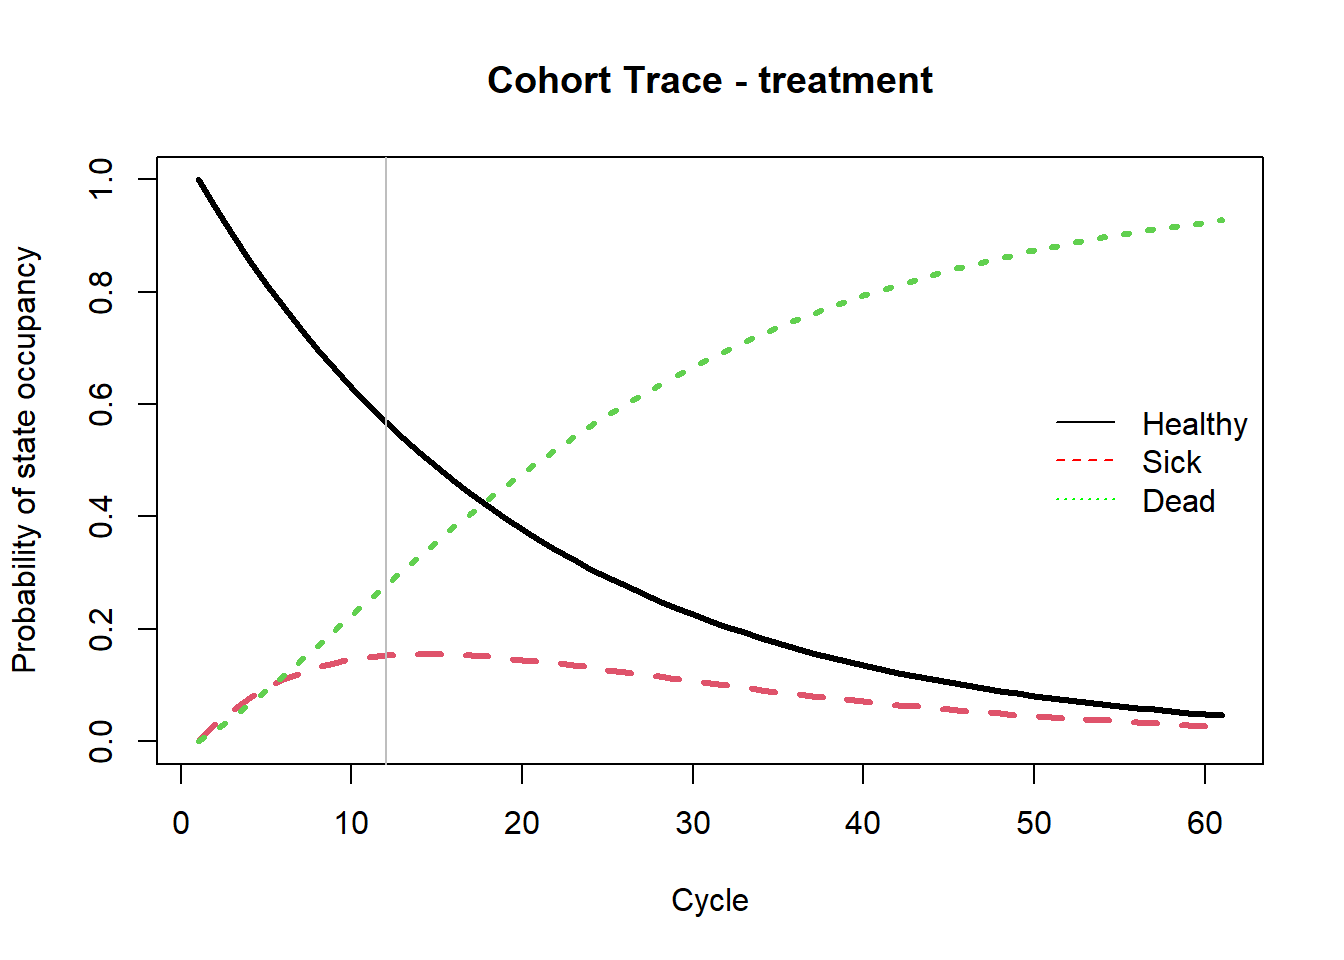
\includegraphics{CRS_Calib_IMIS_files/figure-latex/unnamed-chunk-11-1.pdf}

\begin{Shaded}
\begin{Highlighting}[]
\CommentTok{# TARGET 2: (if you had more...)}
\CommentTok{# plotrix::plotCI(x = lst_targets$Target2$time, y = lst_targets$Target2$value, }
\CommentTok{#                 ui = lst_targets$Target2$ub,}
\CommentTok{#                 li = lst_targets$Target2$lb,}
\CommentTok{#                 ylim = c(0, 1), }
\CommentTok{#                 xlab = "Time", ylab = "Target 2")}
\CommentTok{# points(x = lst_targets$Target2$time, }
\CommentTok{#        y = v_out_best$Target2, }
\CommentTok{#        pch = 8, col = "red")}
\CommentTok{# legend("topright", }
\CommentTok{#        legend = c("Target", "Model-predicted output"),}
\CommentTok{#        col = c("black", "red"), pch = c(1, 8))}
\end{Highlighting}
\end{Shaded}

\end{document}
